\chapter{Web aplikacija}

Svi podaci koji su pohranjeni u bazi podataka trebaju biti korisnicima na raspolaganju jednostavno i intuitivno. U tu je svrhu kreirana aplikacija radi prikaza i vizualizacije podataka korisnicima u stvarnom vremenu. Web aplikacija treba biti javno dostupna na internetu kako bi korisnici razvijenog sustava mogli pregledavati podatke poslane s uređaja. Za objavu web aplikacije na internet \engl{deployment} kreirani su vlastiti resursi na kojima se izvršava aplikacija. Za infrastrukturu aplikacije korišteni su resursi platforme AWS koji pružaju iznajmljivanje virtualnih računala te se na njima mogu pokrenuti vlastite računalne aplikacije. Za web aplikaciju koja će korisnicima pružati uvid u podatke odabrana je Grafana koja nudi brojne funkcionalnosti za vizualizaciju podataka. Nadalje, kreiran je i alarmni sustav koji obavještava o promjenama stanje koja dolaze od uređaja. 

\section{Infrastruktura aplikacije}

Temelj cijele infrastrukture aplikacije jest usluga Amazon EC2 \engl{Elastic Compute Cloud}. Ova usluga pruža skalabilni računalni kapacitet na zahtjev u oblaku platforme AWS. Ova usluga omogućava pokretanje neograničenog broja virtualnih poslužitelja, ovisno o zahtjevima aplikacije i razvijanog sustava, konfiguriranje sigurnosti i umrežavanja te upravljanje pohranom. Usluga EC2 nudi razne prednosti \cite{aws_docs}:
\begin{itemize}
	\item fleksibilno skaliranje: omogućava brzo povećanje ili smanje kapaciteta u kombinaciji s uslugom EC2 Auto Scaling za automatsko skaliranje radi prilagodbe troškova,
	\item potpuna kontrola nad instancom: pruža pristup instanci kao i bilo kojem stroju, moguće pokretanje i zaustavljanje spajanjem na udaljeno računalo, ali i API pozivom,
	\item fleksibilne usluge objave u oblaku: nudi izbor između više vrsta instanci, operacijskih sustava i softverskih paketa te nudi konfiguraciju memorije, procesora i pohrane,
	\item integracija s drugim uslugama: jednostavno se integrira s ostalim uslugama us sklopu platforme AWS,
	\item pouzdanost: nudi vrlo pouzdano okruženje u kojem se zamjenske instance mogu brzo pokrenuti, te je obaveza ugovora o razini usluge Amazon EC2 \engl{Service Level Agreement - SLA} dostupnost od 99,99\% za svaku regiju,
	\item sigurnost: arhitektura nudi različite sigurnosne značajke i postavljanje virtualnih privatnih mreža za ograničen pristup resursima.
\end{itemize}

EC2 instance virtualni su poslužitelji koji rade na infrastrukturi računalstva u oblaku tvrtke Amazon. Jedan fizički AWS poslužitelj uslužuje više EC2 virtualnih poslužitelja koje pokreće hipervizor na računalu domaćinu. Ova usluga pružanja virtualne infrastrukture dio je skupa IaaS usluga koje AWS nudi. EC2 virtualni poslužitelji kopije su izvornog predloška na kojem se temelje. AMI \engl{Amazon Machine Image} temeljna je komponenta koja omogućava pokretanje virtualnih poslužitelja u AWS infrastrukturi. Predstavlja virtualni stroj koji sadrži sve potrebne informacije za pokretanje instance, uključujući operacijski sustav, aplikacije te konfiguracijske podatke. To je prilagodljivi predložak za EC2 instance. Iz jednog AMI predloška, odnosno slike stroja, moguće je kreirati više istih EC2 instanci, što olakšava njihovo stvaranje i objavu na internet. Ovo je korisno za horizontalno skaliranje aplikacija. Slika \ref{fig:ami} prikazuje način na koji funkcionira AMI predložak - kreira instance bilo koje vrste te ih pokrene na domaćinskim računalima \cite{ec2}.

\begin{figure}[ht]
	\centering
	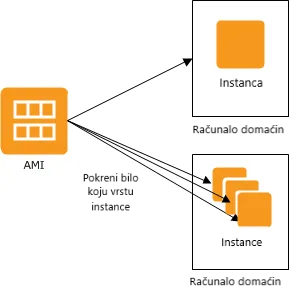
\includegraphics[scale=0.6]{imgs/ami}
	\caption{AMI predložak i distribucija slika stroja na instance \cite{ec2}}
	\label{fig:ami}
\end{figure}

AMI predlošci podržavaju dva tipa virtualizacije: hardversku virtualizaciju i paravirtualizaciju. Predložak s hardverskom virtualizacijom pruža mogućnost pokretanja operacijskog sustava izravno na vrhu virtualnog stroja bez ikakvih izmjena, kao da se pokreće na samom hardveru \engl{bare-metal hardware}. Domaćinski sustav usluge EC2 emulira dio ili sav temeljni hardver koji je predstavljen gostu odnosno AMI slici. Moguće je isto tako koristiti hardverska proširenja koji pružaju brzi pristup domaćinskom hardveru. Paravirtualizacija koristi poseban pokretački program koji lančano učitava jezgru u AMI sliku. Paravirtualni gosti mogu se pokretati na domaćinskom hardveru koji nema eksplicitnu podršku za virtualizaciju. Ovaj tip ne simulira hardver, nego pravi hiperpozive \engl{hypercalls} za izvršavanje osjetljivih CPU naredbi. Preporuča se odabir hardverske virtualizacije, iako generalno paravirtualizacija pruža bolje performanse, zbog poboljšanja hardverske virtualizacije i novih upravljačkih programa koji izjednačava rad obje vrste virtualizacije. 

Pri kreiranju instance potrebno je definirati i njezinu vrstu. Vrsta koja se navede određuje hardver dostupan instanci. Svaka vrsta nudi različitu ravnotežu računalnih, memorijskih i mrežnih resursa. Vrste su grupirane u skupine na temelju potreba ciljnih aplikacija. AWS pruža sljedeće vrste instanci:
\begin{itemize}
	\item opće namjene \engl{general purpose}, 
	\item optimiziranog računanja \engl{compute optimized},
	\item optimizirane memorije \engl{memeory optimized},
	\item optimizirane pohrane \engl{storage optimized}, 
	\item ubrzanog računanja \engl{accelerated computing},
	\item računanje visokih performansi \engl{high-performance computing}.
\end{itemize}

Vrstu instance potrebno je odabrati na temelju zahtjeva same aplikacije. Isto tako, pri kreiranju instance, uvijek je potrebno voditi računa o odabiru regije - optimalno je odabrati regiju kojoj je klijentski promet najbliži.

Za potrebe razvijenog sustava, kreirana je EC2 instanca opće namjene s najmanjim resursima budući da je klijentski promet jako malen, odnosno vrlo malo korisnika treba pristup aplikaciji. Operacijski sustav na kreiranoj instanci je Linux radi lakšeg spajanja na instancu i pokretanja web aplikacije putem komandne linije. Pri stvaranju instance kreirana je nova sigurnosna grupa koja omogućava spajanje na virtualno računalo putem SSH klijenta.

%%TODO finish this

Kako bi se maksimalno izoliralo izvođenje aplikacije i tako ostavilo prostora za izvršavanje drugih procesa na virtualnom računalu, aplikacija je pokrenuta pomoću Dockera. Sljedeći programski isječak prikazuje naredbu za preuzimanje i pokretanje Docker slike za Grafanu. Isto tako, potrebno je izložiti vrata na kojoj se pokreće aplikacija kako bi joj se moglo pristupiti. 

\begin{lstlisting}[caption={Pokretanje Docker slike za Grafanu}, language=bash]
docker run -d -p 3000:3000 --name=grafana grafana/grafana-oss
\end{lstlisting}

%%TODO finish this

Instanci je automatski dodijeljena virtualna privatna mreža \engl{Virtual Private Cloud - VPC} koja predstavlja izolirani virtualni mrežni prostor unutar AWS infrastrukture. Omogućava potpunu kontrolu nad mrežnim okruženjem, uključujući izbor vlastitog IP adresnog prostora, konfiguraciju podmreža, postavljanje usmjeravanja i pristupnih kontrola mreže. Svaka je virtualna privatna mreža podijeljena na manje dijelove mreže zvane podmreže. One mogu biti privatne ili javne. 



%Ovdje opisati stvaranje mrežnog.. nečeg u AWS-u, load balancing i sve što sam već morala kreirati da bih podigla samu aplikaciju na koliko-toliko siguran način. Spomeni povezivanje na SSH i docker i sve. Ipak to spada pod infrastrukturu. 

\section{Grafana}

Gotovo sigurno ću koristiti Grafanu budući da ima gotove vizualizacije koje su meni potrebne. Isto tako, malo opisati funkcionalnosti koje se nude u samoj Grafani, kako funkcionira alerting sustav. Napraviti nekoliko dashboarda, povezati s datasourceom, kreirati par alerta i pokazati kak su došli u obliku maila. Ponuditi proširenja za to - PagerDuty aplikacija recimo.